\documentclass[12pt]{article}
\title{Cardinality}
\author{}
\date{\vspace{-24mm}}
\usepackage[utf8]{inputenc}
\usepackage{amsmath}
\usepackage{amsthm}
\usepackage{geometry}
\usepackage{amsfonts}
\usepackage{mathrsfs}
\usepackage{bm}
\usepackage{hyperref}
\usepackage{xcolor}
\usepackage{enumitem}
\usepackage{changepage}
\usepackage{tikz}
\usetikzlibrary{matrix}
\usepackage{tikz-cd}
\usepackage[nameinlink]{cleveref}
\geometry{
headheight=15pt,
left=60pt,
right=60pt
}
\usepackage{fancyhdr}
\pagestyle{fancy}
\fancyhf{}
\lhead{}
\chead{Cardinality}
\rhead{\thepage}

\hypersetup{
    colorlinks=true,
    linkcolor=blue,
    urlcolor=blue
}

\newcommand{\newp}{\vspace{5mm}}

\theoremstyle{definition}
\newtheorem{definition}{Definition}
\newtheorem{proposition}[definition]{Proposition}
\newtheorem{corollary}[definition]{Corollary}

\newtheorem*{remark}{Remark}

\begin{document}

\maketitle

\tableofcontents

\newpage

\begin{remark}
    \( \mathbb{N} = \{ 1, 2, 3, \ldots \} \).
\end{remark}

\noindent The following is mostly paraphrased from Chapter 2 of \hyperlink{pma}{[PMA]} and Sections 1.5 and 1.6 of \hyperlink{ua}{[UA]}.

\section{Definition of cardinality}
\label{sec:definition_of_cardinality}

\begin{definition}
\label{def:cardinality}
    Let \( A \) and \( B \) be sets. Define a relation \( \sim \) by declaring that \( A \sim B \) if there exists a bijection between \( A \) and \( B \); it is clear that \( \sim \) is an equivalence relation. We say that \( A \) and \( B \) have the same \textbf{cardinality} if and only if \( A \sim B \).
    \begin{enumerate}[label = (\roman*)]
        \item If \( A \sim \{ 1, \ldots, n \} \) for some \( n \in \mathbb{N} \), then we say that \( A \) is \textbf{finite}. In this case, the cardinality or ``size" of \( A \) is simply the number of elements belonging to \( A \) and we write \( |A| = n \). We also take the empty set to be finite and consider it to contain zero elements.

        \item If \( A \) is not finite, then we say that \( A \) is \textbf{infinite}.

        \item If \( A \sim \mathbb{N} \), then we say that \( A \) is \textbf{countably infinite, countable, denumerable,} or \textbf{enumerable}.

        \item If \( A \)  is finite or countably infinite, we say that \( A \) is \textbf{at most countable}.

        \item If \( A \) is infinite but not countably infinite, we say that \( A \) is \textbf{uncountably infinite} or \textbf{uncountable}.
    \end{enumerate}
\end{definition}

\section{Countable infinities}
\label{sec:countable_infinities}

\begin{proposition}
\label{prop:Z_is_countable}
    \( \mathbb{Z} \) is countably infinite.
\end{proposition}

\begin{proof}
    Define functions \( f : \mathbb{N} \to \mathbb{Z} \) and \( g : \mathbb{Z} \to \mathbb{N} \) as follows:
    \[
    f(n) = \begin{cases}
        \frac{n}{2} & \text{if } n \text{ is even}, \\
        -\frac{n-1}{2} & \text{if } n \text{ is odd},
    \end{cases}
    \qquad \text{and} \qquad
    g(k) = \begin{cases}
        2k & \text{if } k > 0, \\
        -2k + 1 & \text{if } k \leq 0.
    \end{cases}
    \]

    \[
    \begin{tikzcd}[column sep = tiny, row sep = small]
        \mathbb{N} : & 1 \arrow[d, leftrightarrow] & 2 \arrow[d, leftrightarrow] & 3 \arrow[d, leftrightarrow] & 4 \arrow[d, leftrightarrow] & 5 \arrow[d, leftrightarrow] & \cdots \\
        \mathbb{Z} : & 0 & 1 & -1 & 2 & -2 & \cdots \\
    \end{tikzcd}
    \]
    It is straightforward to verify that \( f \) and \( g \) are mutual inverses.
\end{proof}

\begin{proposition}
\label{prop:infinite_subset_of_countable_set_is_countable}
    Suppose \( A \) is countably infinite and \( B \subseteq A \) is infinite. Then \( B \) is countably infinite.
\end{proposition}

\begin{proof}
    Since \( A \) is countably infinite, there exists a bijection \( f : \mathbb{N} \to A \). We will inductively construct a bijection \( g : \mathbb{N} \to B \) as follows. Since \( B \) is non-empty, \( f^{-1}(B) \) is also non-empty, so we may set \( n_1 = \min( f^{-1}(B)) \). Suppose that after \( k \) steps we have chosen positive integers \( n_1 < \cdots < n_k \) such that
    \[
        n_1 = \min(f^{-1}(B)), \quad n_i = \min(f^{-1}(B) \setminus \{ n_1, \ldots, n_{i-1} \}) \text{ for } 2 \leq i \leq k.
    \]
    We claim that the set \( E := f^{-1}(B) \setminus \{ n_1, \ldots, n_k \} \) is non-empty; indeed, \( E \) must be infinite. Since \( f \) is a bijection, we have
    \[
        B = f(f^{-1}(B)) = f(E \cup \{ n_1, \ldots, n_k \}) = f(E) \cup f(\{n_1, \ldots, n_k\}).
    \]
    Evidently: \( f(\{n_1, \ldots, n_k\} \) is a finite set; the union of two finite sets is again a finite set; and \( E \sim f(E) \) via \( f \). Hence \( E \) being finite implies that \( B \) is finite; by the contrapositive we see that \( E \) must be infinite. We are then justified in setting \( n_{k+1} = \min( f^{-1}(B) \setminus \{ n_1, \ldots, n_k \} ) \). In this way we obtain a sequence \( n_1 < \cdots < n_k < \cdots \) of positive integers such that
    \[
        n_1 = \min(f^{-1}(B)), \quad n_k = \min(f^{-1}(B) \setminus \{ n_1, \ldots, n_{k-1} \}) \text{ for } 2 \leq k.
    \]
    We define \( g \) by setting \( g(k) = f(n_k) \in B \). Observe that since \( f \) is injective we have
    \[
        g(k) = g(l) \iff f(n_k) = f(n_l) \iff n_k = n_l.
    \]
    Suppose that \( k < l \). Then \( n_k < n_l \); it follows that \( g \) is injective. To see that \( g \) is surjective, let \( b \in B \) be given. Since \( f \) is surjective, there is a positive integer \( N \) such that \( f(N) = b \). Suppose that for all \( k \in \mathbb{N} \) we have \( N \neq n_k \). It cannot be the case that \( N < n_1 \), else \( n_1 \) would not be the minimum of \( f^{-1}(B) \), so we must have \( n_1 < N \). Then the set \( \{ k \in \mathbb{N} : n_k < N \} \) is non-empty and finite (it contains at most \( N - 1 \) elements), so \( l := \max \{ k \in \mathbb{N} : n_k < N \} \) exists and we have \( n_l < N < n_{l+1} \); but this contradicts \( n_{l+1} \) being the minimum of the set \( f^{-1}(B) \setminus \{ n_1, \ldots, n_l \} \). So in fact there must exist a \( k \in \mathbb{N} \) such that \( n_k = N \) and it follows that \( g(k) = f(n_k) = f(N) = b \).
\end{proof}

\begin{proposition}
\label{prop:countable_iff_surjection_from_N}
    A set \( A \) is countably infinite if and only if \( A \) is infinite and there exists a surjection \( f : \mathbb{N} \to A \).
\end{proposition}

\begin{proof}
    A bijection is in particular a surjection, so the forward implication is clear. For the converse implication, suppose there exists a surjection \( f : \mathbb{N} \to A \). Then \( f^{-1} \{ a \} \) is non-empty for any \( a \in A \), so the function \( g : A \to \mathbb{N} \) given by \( g(a) = \min( f^{-1} \{ a \} ) \) is well-defined. This function is injective since
    \[
        g(a_1) = g(a_2) \implies f(g(a_1)) = f(g(a_2)) \iff a_1 = a_2.
    \]
    Hence we see that \( A \sim g(A) \) via \( g \). Since \( A \) is infinite, \( g(A) \) must also be infinite. Then by \Cref{prop:infinite_subset_of_countable_set_is_countable}, \( g(A) \sim \mathbb{N} \). It follows that \( A \sim \mathbb{N} \), i.e.\ \( A \) is countably infinite.
\end{proof}

\begin{proposition}
\label{prop:countable_union_of_countable_sets_is_countable}
    Suppose for each \( n \in \mathbb{N} \) we have a countably infinite set \( A_n \). Then the union \( \bigcup_{n=1}^{\infty} A_n \) is countably infinite.
\end{proposition}

\begin{proof}
    By \Cref{prop:countable_iff_surjection_from_N}, it will suffice to construct a surjection \( g : \mathbb{N} \to \bigcup_{n=1}^{\infty} A_n \). For each \( n \in \mathbb{N} \) we have a bijection \( f_n : \mathbb{N} \to A_n \). For \( m, n \in \mathbb{N} \), let \( a_{mn} = f_n(m) \). As a sketch of our construction, arrange these terms in an ``infinite grid'' like so:
    \[
        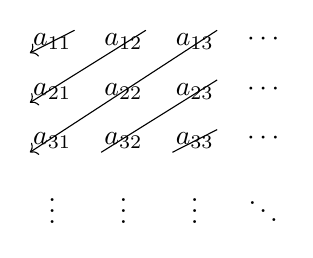
\begin{tikzpicture}
            \matrix[matrix of math nodes,inner sep=1pt,row sep=1em,column sep=1em] (M)
            {
                a_{11} & a_{12} & a_{13} & \cdots \\
                a_{21} & a_{22} & a_{23} & \cdots \\
                a_{31} & a_{32} & a_{33} & \cdots \\
                \vdots & \vdots & \vdots & \ddots \\
            }
            ;
            \draw[->] (M-1-1.north east) -- (M-1-1.south west);
            \draw[->] (M-1-2.north east) -- (M-2-1.south west);
            \draw[->] (M-1-3.north east) -- (M-3-1.south west);
            \draw[-] (M-2-3.north east) -- (M-3-2.south west);
            \draw[-] (M-3-3.north east) -- (M-3-3.south west);
        \end{tikzpicture}
    \]
    We define \( g \) by working our way through the grid along the diagonals as shown in the infinite grid, setting \( g(1) = a_{11}, g(2) = a_{12}, g(3) = a_{21}, g(4) = a_{13}, g(5) = a_{22}, g(6) = a_{31} \), and so on. Since each \( f_n \) is in particular a surjection, each element of \( \bigcup_{n=1}^{\infty} A_n \) appears somewhere in this grid, lying on some diagonal. It follows that \( g \) is a surjection. To give an explicit construction of \( g \) is tedious and not particularly illuminating, but nonetheless we will do so.

    \vspace{2mm}

    \noindent To be explicit then, for \( n \in \mathbb{N} \), let \( t_n = \tfrac{n(n-1)}{2} \), so that \( t_1 = 0, t_2 = 1, t_3 = 3, t_4 = 6, \) and so on. Let \( k \in \mathbb{N} \) be given. The set \( T_k = \{ m \in \mathbb{N} : t_m < k \} \) is non-empty (\( t_1 \in T_k \)) and finite (it could contain at most \( k - 1 \) elements), so \( n := \max T_k \) exists; it follows that \( t_n < k \leq t_{n+1} \). Conversely, if \( t_n < k \leq t_{n+1} \) for some \( n \in \mathbb{N} \), then \( n = \max T_k \). Given this, setting
    \[
        g(k) = a_{k - t_n,t_{n+1} + 1 - k} = f_{t_{n+1} + 1 - k}(k - t_n)
    \]
    gives us a well-defined function \( g : \mathbb{N} \to \bigcup_{n=1}^{\infty} A_n \). To see that \( g \) is surjective, let \( a \in \bigcup_{n=1}^{\infty} A_n \) be given. Then \( a \in A_n \) for some \( n \in \mathbb{N} \). Since \( f_n \) is a surjection, there exists \( m \in \mathbb{N} \) such that \( a = f_n(m) = a_{mn} \). Let \( k = t_{m + n - 1} + m \). Observe that
    \[
        k \leq t_{m+n} \iff \frac{(m+n-1)(m+n-2)}{2} + m \leq \frac{(m+n)(m+n-1)}{2} \iff m \leq m + n - 1.
    \]
    The statement \( m \leq m + n - 1 \) is certainly true, so we see that \( t_{m+n-1} < k \leq t_{m+n} \). It follows that \( \max T_k = m + n - 1 \). Then \( k - t_{m+n-1} = m \) and
    \begin{align*}
        t_{m+n} + 1 - k &= t_{m+n} - t_{m+n-1} - m + 1 \\
        &= \frac{(m+n)(m+n-1)}{2} - \frac{(m+n-1)(m+n-2)}{2} - m + 1 \\
        &= m + n - 1 - m + 1 \\
        &= n.
    \end{align*}
    Hence \( g(k) = a_{mn} = a \).
\end{proof}

\begin{corollary}
\label{cor:union_of_amc_set_and_countable_set_is_countable}
    Suppose we have an at most countable set \( A \) and a countably infinite set \( B \). Then \( A \cup B \) is countably infinite.
\end{corollary}

\begin{proof}
    \begin{enumerate}[label = (\roman*)]
        \item Suppose that \( A \) is finite, say \( A = \{ a_1, \ldots, a_k \} \) for some \( k \in \mathbb{N} \). By \Cref{prop:countable_iff_surjection_from_N}, there is a surjection \( f : \mathbb{N} \to B \). Define a function \( g : \mathbb{N} \to A \cup B \) by
        \[
            g(1) = a_1, \ldots, g(k) = a_k, \text{ and  } g(n) = f(n - k) \text{ for } n > k.
        \]
        Then \( g \) is a surjection and we may invoke \Cref{prop:countable_iff_surjection_from_N} to conclude that \( A \cup B \) is countably infinite.

        \item Suppose that \( A \) is countably infinite. This is then a special case of \Cref{prop:countable_union_of_countable_sets_is_countable}. Indeed, take \( E_1 = A \) and \( E_n = B \) for \( n \geq 2 \); then each \( E_n \) is countably infinite and
        \[
            A \cup B = \bigcup_{n=1}^{\infty} E_n.
        \]
        \Cref{prop:countable_union_of_countable_sets_is_countable} then implies that \( A \cup B \) is countably infinite. \qedhere
    \end{enumerate}
\end{proof}

\begin{proposition}
\label{prop:amc_union_of_amc_sets_is_amc}
    Suppose we have some at most countable indexing set \( I \) and, for each \( i \in I \), an at most countable set \( A_i \).
    \begin{enumerate}[label = (\roman*)]
        \item If \( I \) is finite and each \( A_i \) is finite, then \( \bigcup_{i \in I} A_i \) is finite.
        
        \item If \( I \) is countably infinite and there is a finite subset \( J \subseteq I \) such that \( A_i \) is finite for \( i \in J \) and \( A_i \) is empty for \( i \not\in J \), then \( \bigcup_{i \in I} A_i \) is finite. (This includes the possibility that each \( A_i \) is empty.)
        
        \item If at least one \( A_i \) is countably infinite, then \( \bigcup_{i \in I} A_i \) is countably infinite.

        \item If \( I \) is countably infinite and there is an infinite subset \( J \subseteq I \) such that \( A_i \) is finite and non-empty for \( i \in J \) and \( A_i \) is empty for \( i \not\in J \), then \( \bigcup_{i \in I} A_i \) is at most countable.
    \end{enumerate}
    These cases are exclusive and exhaustive. In any case, \( \bigcup_{i \in I} A_i \) is at most countable; we can never obtain an uncountably infinite set by taking at most countable unions of at most countable sets.
\end{proposition}

\begin{proof}
    \begin{enumerate}[label = (\roman*)]
        \item \( \bigcup_{i \in I} A_i \) contains at most \( \sum_{i \in I} |A_i| \) elements; less if the \( A_i \)'s have elements in common. (The exact number of elements in the union is given by the \href{https://en.wikipedia.org/wiki/Inclusion%E2%80%93exclusion_principle}{inclusion-exclusion principle}.)

        \item We have \( \bigcup_{i \in I} A_i = \bigcup_{i \in J} A_i \); now apply part (i).

        \item Suppose \( A_j \) is countably infinite for some \( j \in I \). If \( I \) is finite, say \( \{ 1, \ldots, k \} \sim I \) via some bijection \( f \), let \( E_n = A_{f(n)} \cup A_j \) for \( 1 \leq n \leq k \) and \( E_n = A_j \) for \( n > k \). If \( I \) is countably infinite, let \( f : \mathbb{N} \to I \) be a bijection, and define \( E_n = A_{f(n)} \cup A_j \) for \( n \in \mathbb{N} \). In either case, by \Cref{cor:union_of_amc_set_and_countable_set_is_countable}, each \( E_n \) is countably infinite. Furthermore,
        \[
            \bigcup_{i \in I} A_i = \bigcup_{n=1}^{\infty} E_n.
        \]
        The result now follows from \Cref{prop:countable_union_of_countable_sets_is_countable}.

        \item For \( i \in J \), let \( E_i = A_i \cup \mathbb{N} \). Then each \( E_i \) is countably infinite by \Cref{cor:union_of_amc_set_and_countable_set_is_countable} and
        \[
            \bigcup_{i \in I} A_i = \bigcup_{i \in J} A_i \subseteq \bigcup_{i \in J} E_i.
        \]
        \( J \) is countably infinite by \Cref{prop:infinite_subset_of_countable_set_is_countable}, so we may apply part (iii) to see that \( \bigcup_{i \in J} E_i \) is countably infinite. If \( \bigcup_{i \in J} A_i \) is finite, we are done. If it is infinite, then the desired result follows from \Cref{prop:infinite_subset_of_countable_set_is_countable}. \qedhere
    \end{enumerate}
\end{proof}

\begin{remark}
    In part (iv) of \Cref{prop:amc_union_of_amc_sets_is_amc}, it may be the case that \( \bigcup_{i \in J} A_i \) is finite or countably infinite. For two examples, consider \( A_i = \{ 0 \} \) for each \( i \in \mathbb{N} \). Then \( \bigcup_{i=1}^{\infty} A_i = \{ 0 \} \), a finite set. Now consider \( A_i = \{ i \} \) for each \( i \in \mathbb{N} \). Then \( \bigcup_{i=1}^{\infty} A_i = \mathbb{N} \), a countably infinite set.
\end{remark}

\begin{corollary}
\label{cor:finite_product_of_amc_sets_is_amc}
    Suppose we have finitely many at most countable sets \( A_1, \ldots, A_n \).
    \begin{enumerate}[label = (\roman*)]
        \item If each \( A_i \) is finite, then \( \prod_{i=1}^n A_i \) is finite (where \( \prod_{i=1}^n A_i \) is the Cartesian product \( A_1 \times \cdots \times A_n \)).

        \item If each \( A_i \) is non-empty and at least one \( A_i \) is countably infinite, then \( \prod_{i=1}^n A_i \) is countably infinite.
    \end{enumerate}
\end{corollary}

\begin{proof}
    \begin{enumerate}[label = (\roman*)]
        \item \( \prod_{i=1}^n A_i \) has exactly \( \prod_{i=1}^n |A_i| \) elements.

        \item First, let us prove the special case where each \( A_i \) is countably infinite. For the base case, suppose we have countably infinite sets \( A_1 \) and \( A_2 \). Let \( f : \mathbb{N} \to A_2 \) be a bijection. For any fixed \( a \in A_1 \), we have \( \mathbb{N} \sim (\{ a \} \times A_2) \) via the map \( n \mapsto (a, f(n)) \). Observe that
        \[
            A_1 \times A_2 = \bigcup_{a \in A_1} (\{ a \} \times A_2).
        \]
        Hence \( A_1 \times A_2 \) is countably infinite by \Cref{prop:amc_union_of_amc_sets_is_amc} (iii). The special case now follows by induction. For the general case, suppose \( A_j \) is countably infinite for some \( 1 \leq j \leq n \). Let \( E_i = A_i \cup A_j \) for \( 1 \leq i \leq n \). Then each \( E_i \) is countably infinite by \Cref{cor:union_of_amc_set_and_countable_set_is_countable} and so the product \( \prod_{i=1}^n E_i \) is also countably infinite by the special case we just proved. Furthermore,
        \[
            \prod_{i=1}^n A_i \subseteq \prod_{i=1}^n E_i.
        \]
        Since each \( A_i \) is non-empty, there exists \( a_i \in A_i \) for each \( 1 \leq i \leq n \). Then the infinite set \( \{ a_1 \} \times \cdots \times A_j \times \cdots \times \{ a_n \} \) is contained in \( \prod_{i=1}^n A_i \). It follows that \( \prod_{i=1}^n A_i \) is infinite and so by \Cref{prop:infinite_subset_of_countable_set_is_countable} we may conclude that \( \prod_{i=1}^n A_i \) is countably infinite. \qedhere
    \end{enumerate}
\end{proof}

\begin{remark}
    \Cref{cor:finite_product_of_amc_sets_is_amc} cannot be generalised to the product of infinitely many sets, i.e.\ the product of infinitely many at most countable sets need not be at most countable -- even if the factors are finite! We shall give a counterexample in \Cref{prop:no_surjection_from_N_to_set_of_binary_sequences}.
\end{remark}

\begin{corollary}
\label{cor:Q_is_countable}
    \( \mathbb{Q} \) is countably infinite.
\end{corollary}

\begin{proof}
    Let us take as our construction of \( \mathbb{Q} \) the set of equivalence classes of elements in \( \mathbb{Z} \times (\mathbb{Z} \setminus \{ 0 \}) \) where we declare \( (a, b) \) and \( (c, d) \) equivalent if and only if \( ad = bc \). Let \( \pi : \mathbb{Z} \times (\mathbb{Z} \setminus \{ 0 \}) \to \mathbb{Q} \) be the canonical map, which is always a surjection. By \Cref{prop:Z_is_countable}, \( \mathbb{Z} \) is countably infinite; it is straightforward to modify the proof of that proposition to see that \( \mathbb{Z} \setminus \{ 0 \} \) is also countably infinite. Then by \Cref{cor:finite_product_of_amc_sets_is_amc}, \( \mathbb{Z} \times (\mathbb{Z} \setminus \{ 0 \}) \) is countably infinite. Let \( f : \mathbb{N} \to \mathbb{Z} \times (\mathbb{Z} \setminus \{ 0 \}) \) be a bijection. Then the composition \( \pi \circ f : \mathbb{N} \to \mathbb{Q} \) is a surjection and hence by \Cref{prop:countable_iff_surjection_from_N} we see that \( \mathbb{Q} \) is countably infinite.
\end{proof}

\section{Power sets}
\label{sec:power_sets}

For a set \( A \), we will write \( \mathscr{P}(A) \) for the \href{https://en.wikipedia.org/wiki/Power_set}{power set} of \( A \).

\begin{proposition}
\label{prop:bijection_between_sets_implies_bijection_between_power_sets}
    Suppose we have sets \( A \) and \( B \) such that \( A \sim B \). Then \( \mathscr{P}(A) \sim \mathscr{P}(B) \).
\end{proposition}

\begin{proof}
    Let \( f : A \to B \) be a bijection. We define two functions \( F : \mathscr{P}(A) \to \mathscr{P}(B) \) and \( G : \mathscr{P}(B) \to \mathscr{P}(A) \) by
    \[
        F(X) = \{ f(x) : x \in X \} \qquad \text{and} \qquad G(Y) = \{ f^{-1}(y) : y \in Y \}.
    \]
    It is straightforward to verify that \( F \) and \( G \) are mutual inverses.
\end{proof}

\begin{proposition}[Cantor's theorem]
\label{prop:no_surjection_from_set_to_power_set}
    Let \( A \) be a set and \( f : A \to \mathscr{P}(A) \) a function. Then \( f \) is not a surjection.
\end{proposition}

\begin{proof}
    Let \( B = \{ x \in A : x \not\in f(x) \} \in \mathscr{P}(A) \) (this set is sometimes called the Cantor diagonal set of \( f \)). Suppose \( f \) is a surjection, so that there exists some \( x \in A \) such that \( f(x) = B \). Then \( x \in B \iff x \not\in f(x) = B \), a contradiction. It follows that \( f \) cannot be a surjection.
\end{proof}

\section{Uncountable infinities}
\label{sec:uncountable_infinities}

\begin{proposition}
\label{prop:no_surjection_from_N_to_set_of_binary_sequences}
    Let \( T \) be the set of all binary sequences, i.e.\
    \[
        T = \prod_{n=1}^{\infty} \{ 0, 1 \} = \{ (x_1, x_2, x_3, \ldots) : x_n \in \{ 0, 1 \} \},
    \]
    and let \( f : \mathbb{N} \to T \) be a function. Then \( f \) is not a surjection.
\end{proposition}

\begin{proof}
    For each \( n \in \mathbb{N} \), let \( x_n = 0 \) if \( f(n) = 1 \) and let \( x_n = 1 \) if \( f(n) = 0 \). Then the sequence \( \bm{x} = (x_1, x_2, x_3, \ldots) \) cannot possibly belong to the image \( f(\mathbb{N}) \) since it differs from each \( f(n) \) in the \( n \)th position. It follows that \( f(\mathbb{N}) \neq T \), i.e.\ that \( f \) is not a surjection.
\end{proof}

\Cref{prop:no_surjection_from_N_to_set_of_binary_sequences} implies that the set of all binary sequences \( T \) cannot be put in bijection with \( \mathbb{N} \); since \( T \) is evidently infinite, it follows that \( T \) is uncountably infinite.

\begin{proposition}
\label{prop:set_of_binary_sequences_in_bijection_with_power_set_of_naturals}
    \( \mathscr{P}(\mathbb{N}) \) has the same cardinality as \( T \).
\end{proposition}

\begin{proof}
    Define a function \( f : \mathscr{P}(\mathbb{N}) \to T \) by mapping a subset \( E \subseteq \mathbb{N} \) to the binary sequence \( (a_1, a_2, a_3, \ldots) \), where \( a_n = 1 \) if \( n \in E \) and \( a_n = 0 \) if \( n \not\in E \), and define a function \( g : T \to \mathscr{P}(\mathbb{N}) \) by mapping a sequence \( (a_1, a_2, a_3, \ldots) \) to the subset \( E = \{ n \in \mathbb{N} : a_n = 1 \} \). It is straightforward to verify that \( f \) and \( g \) are mutual inverses.
\end{proof}

\begin{remark}
    We could have proved \Cref{prop:no_surjection_from_N_to_set_of_binary_sequences} by combining \Cref{prop:no_surjection_from_set_to_power_set} (Cantor's theorem) with \Cref{prop:set_of_binary_sequences_in_bijection_with_power_set_of_naturals}.
\end{remark}

Let us now consider the cardinality of \( \mathbb{R} \). Using the binary representation of real numbers, one can construct a bijection between \( \mathbb{R} \) and the set of all binary sequences \( T \). \Cref{prop:no_surjection_from_N_to_set_of_binary_sequences} then implies that \( \mathbb{R} \) is uncountably infinite. However, we will take a different approach, using the \href{https://lew98.github.io/Mathematics/Miscellaneous/Nested_interval_property.pdf}{nested interval property} of \( \mathbb{R} \), which is much closer to Cantor's original 1874 proof of the uncountability of \( \mathbb{R} \).

\begin{proposition}
\label{prop:no_surjection_from_N_to_R}
    Let \( f : \mathbb{N} \to \mathbb{R} \) be a function. Then \( f \) is not a surjection.
\end{proposition}

\begin{proof}
    Let \( I_1 = [a_1, b_1] \) be any closed bounded interval which does not contain \( f(1) \); taking \( I_1 = [f(1) + 1, f(1) + 2] \) will do. Let \( m = \frac{2}{3}a_1 + \frac{1}{3}b_1 \) and \( M = \frac{1}{3}a_1 + \frac{2}{3} b_1 \).
    \[
    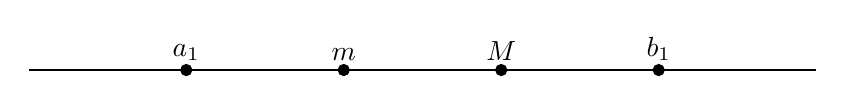
\begin{tikzpicture}
        \draw[black, thick] (0, 0) -- (10, 0);
        \filldraw[black] (2, 0) circle (2pt) node[anchor=south]{$a_1$};
        \filldraw[black] (4, 0) circle (2pt) node[anchor=south]{$m$};
        \filldraw[black] (6, 0) circle (2pt) node[anchor=south]{$M$};
        \filldraw[black] (8, 0) circle (2pt) node[anchor=south]{$b_1$};
    \end{tikzpicture}
    \]
    If \( f(2) \not\in [a_1, m] \), then let \( a_2 = a_1, b_2 = m \), and set \( I_2 = [a_2, b_2] \). If \( f(2) \in [a_1, m] \), then \( f(2) \not\in [M, b_1] \), so let \( a_2 = M, b_2 = b_1 \), and set \( I_2 = [a_2, b_2] \). In either case, \( f(1) \not\in I_1, f(2) \not\in I_2 \), and \( |I_2| = b_2 - a_2 = 3^{-1}(b_1 - a_1) \). Now repeat this argument with \( I_2 \), and then with \( I_3 \), and so on; inductively, we obtain a sequence of shrinking nested intervals \( (I_n)_{n \in \mathbb{N}} \) such that \( f(n) \not\in I_n \) for each \( n \in \mathbb{N} \). By the \href{https://lew98.github.io/Mathematics/Nested_interval_property.pdf}{nested interval property} of \( \mathbb{R} \), there exists an \( x \in \mathbb{R} \) such that \( \bigcap_{n=1}^{\infty} I_n = \{ x \} \). It follows that \( x \) does not belong to the image of \( f \), since \( x = f(n) \) implies that \( f(n) \in I_n \). Hence \( f \) is not a surjection.
\end{proof}

Evidently, \( \mathbb{R} \) is infinite; \Cref{prop:no_surjection_from_N_to_R} then implies that \( \mathbb{R} \) is uncountably infinite. In light of \Cref{cor:union_of_amc_set_and_countable_set_is_countable}, which implies that the union of two countably infinite sets is countably infinite, and \Cref{cor:Q_is_countable}, which says that \( \mathbb{Q} \) is countably infinite, we see that the set of irrational numbers \( \mathbb{R} \setminus \mathbb{Q} \) must be uncountably infinite.

\section{Schröder-Bernstein theorem}
\label{sec:schroder-bernstein_theorem}

\begin{remark}
    In what follows, we will write \( A^{\mathsf{C}} \) for the complement of a set \( A \), i.e.\ \( A^{\mathsf{C}} \) is the set of those \( x \) which do not belong to \( A \).
\end{remark}

\begin{proposition}[Schröder-Bernstein theorem]
\label{prop:schroder-bernstein_theorem}
    Let \( X \) and \( Y \) be sets and suppose we have injective functions \( f : X \to Y \) and \( g : Y \to X \). Then there exists a bijection \( h : X \to Y \).
\end{proposition}

\begin{proof}
    Let \( A_1 = [g(Y)]^{\mathsf{C}}, A_n = g(f(A_{n-1})) \) for \( n \geq 2 \), \( A = \bigcup_{n=1}^{\infty} A_n \), and \( B = \bigcup_{n=1}^{\infty} f(A_n) \). Consider the restriction \( f|_A : A \to B \). From the definitions of \( A \) and \( B \), it is clear that \( f|_A \) indeed maps into \( B \) and in fact is surjective. Since \( f : X \to Y \) is injective, \( f|_A \) is also injective and hence bijective. Now consider the restriction \( g|_{B^{\mathsf{C}}} : B^{\mathsf{C}} \to A^{\mathsf{C}} \). This maps into \( A^{\mathsf{C}} \) since
    \[
        \arraycolsep=1pt\def\arraystretch{1.3}
        \begin{array}{rcl}
            b \in B^{\mathsf{C}} & \iff & \forall n \in \mathbb{N},\, b \not\in f(A_n) \\
            & \iff & \forall n \in \mathbb{N},\, g(b) \not\in g(f(A_n)) \\
            & \iff & \forall n \in \mathbb{N},\, g(b) \not\in A_{n+1} \\
            & \iff & \forall n \geq 2,\, g(b) \not\in A_n. \\
        \end{array}
    \]
    Since \( A_1 \) is the complement of the image of \( Y \) under \( g \), it follows that \( g(y) \not\in A_1 \) for any \( y \in Y \). Hence
    \[
        b \in B^{\mathsf{C}} \iff \forall n \in \mathbb{N},\, g(b) \not\in A_n \iff g(b) \in A^{\mathsf{C}}.
    \]
    Furthermore, \( g|_{B^{\mathsf{C}}} \) is surjective since for any \( a \in A^{\mathsf{C}} \) we have \( a \not\in A_1 \iff a \in g(Y) \), so that \( a = g(y) \) for some \( y \in Y \). The chain of bi-implications above then shows that \( y \in B^{\mathsf{C}} \). Since \( g : Y \to X \) is injective, \( g|_{B^{\mathsf{C}}} \) is also injective and hence bijective. Given this, the functions \( h_1 : X \to Y \) and \( h_2 : Y \to X \) given by
    \[
        h_1(x) = \begin{cases}
            f|_A(x) & \text{ if } x \in A, \\
            g|_{B^{\mathsf{C}}}^{-1}(x) & \text{ if } x \in A^{\mathsf{C}},
        \end{cases}
        \qquad
        h_2(y) = \begin{cases}
            f|_A^{-1}(y) & \text{ if } y \in B, \\
            g|_{B^{\mathsf{C}}}(x) & \text{ if } y \in B^{\mathsf{C}}
        \end{cases}
    \]
    are well-defined and mutual inverses.
\end{proof}

For an application of the Schröder-Bernstein theorem, let us show that \( [0, 1] \sim (0, 1) \). Consider the injections \( f : [0, 1] \to (0, 1) \) and \( g : (0, 1) \to [0, 1] \) given by \( f(x) = \tfrac{1}{2}x + \tfrac{1}{4} \) and \( g(x) = x \). The Schröder-Bernstein theorem then guarantees the existence of a bijection between \( [0, 1] \) and \( (0, 1) \), but furthermore shows us how to find an explicit bijection. Following the procedure detailed in the proof of the theorem, we have \( A_1 = \{ 0, 1 \}, A_2 = \left\{ \tfrac{1}{4}, \tfrac{3}{4} \right\}, A_3 = \left\{ \tfrac{3}{8}, \tfrac{5}{8} \right\} \), and in general \( A_n = \left\{ \tfrac{1}{2} - 2^{-n}, \tfrac{1}{2} + 2^{-n} \right\} \), which gives \( f(A_n) = \left\{ \tfrac{1}{2} - 2^{-n-1}, \tfrac{1}{2} + 2^{-n-1} \right\} \). Then if we define \( h : X \to Y \) by
\[
    h(x) = \begin{cases}
        \tfrac{1}{2}x + \tfrac{1}{4} & \text{if } x \in \bigcup_{n=1}^{\infty} \left\{ \tfrac{1}{2} - 2^{-n}, \tfrac{1}{2} + 2^{-n} \right\}, \\
        x & \text{otherwise},
    \end{cases}
\]
we can be sure that \( h \) is a bijection with inverse
\[
    h^{-1}(y) = \begin{cases}
        2y - \tfrac{1}{2} & \text{if } y \in \bigcup_{n=1}^{\infty} \left\{ \tfrac{1}{2} - 2^{-n-1}, \tfrac{1}{2} + 2^{-n-1} \right\}, \\
        y & \text{otherwise}.
    \end{cases}
\]

\noindent \hrulefill

\noindent \hypertarget{pma}{\textcolor{blue}{[PMA]} Rudin, W. (1976) \textit{Principles of Mathematical Analysis.} 3rd edn.}

\noindent \hypertarget{ua}{\textcolor{blue}{[UA]} Abbott, S. (2015) \textit{Understanding Analysis.} 2nd edn.}

\end{document}
